\documentclass[10pt, conference, letterpaper]{IEEEtran}
\IEEEoverridecommandlockouts
% The preceding line is only needed to identify funding in the first footnote. If that is unneeded, please comment it out.
\usepackage{cite}
\usepackage{amsmath,amssymb,amsfonts}
\usepackage{algorithmic}
\usepackage{graphicx}
\usepackage{textcomp}
\usepackage{xcolor}
\usepackage[T1]{fontenc}

\usepackage{courier} 
\usepackage{epsfig}
\usepackage{subfigure}
\usepackage{multirow}
\usepackage{color}
\usepackage{amsthm}
\usepackage[numbers,sort&compress]{natbib}
\usepackage{comment}

\usepackage{algorithm}

\pagestyle{plain}

\def\BibTeX{{\rm B\kern-.05em{\sc i\kern-.025em b}\kern-.08em
    T\kern-.1667em\lower.7ex\hbox{E}\kern-.125emX}}
\begin{document}

\long\def\tian#1{{\color{blue} \textbf{[Tian: #1]}}}

\newcommand{\tabincell}[2]{\begin{tabular}{@{}#1@{}}#2\end{tabular}}
\newcommand{\eg}{{\it e.g.}}
\newcommand{\aka}{{\it a.k.a.}}
\newcommand{\etal}{{\it et al.}}
\newcommand{\etc}{{\it etc}}
\newcommand{\ie}{{\it i.e.}}

\title{INT-path: Towards Optimal Path Planning for In-band
Network-Wide Telemetry}

\author{\#1570473294, 9 pages}

\maketitle

\begin{abstract}


With the ever-increasing complexity of networks, fine-grained network monitoring enables better network reliability and timely feedback control. The In-band Network Telemetry (INT) allows cost-effective network monitoring by encapsulating device-internal states into probe packets. However, INT only specifies an underlying device-level primitive while how to achieve \emph{network-wide} traffic monitoring remains undefined. In this work, we propose \emph{INT-path}, a network-wide telemetry \emph{framework}, by decoupling the system into a routing mechanism and a routing path generation policy. Specifically, we embed \emph{source routing} into INT probes to allow specifying the route the probe packet takes through the network. Above the mechanism, we develop an \emph{Euler trail-based} path planning policy to generate \emph{non-overlapped} INT paths that cover the entire network with a \emph{minimum} path number and give an exhaustive analysis of algorithm's run-time complexity. INT-path can ``encode'' the network-wide traffic status into a series of ``bitmap images'', transforming network troubleshooting into well-studied pattern recognition problems. INT-path is very suitable for deployment in data center networks thanks to their symmetry network topologies. 

\end{abstract}




\section{Introduction}

Today's data center networks have become mega-scale with increasing deployment of diverse cloud services. With the continuous expansion of network size, fine-grained network monitoring becomes the prerequisite for better network reliability and closed-loop traffic control. In traditional network monitoring, management protocols, such as SNMP~\cite{case1990simple}, are widely adopted to constantly poll the router/switch CPU for collecting device-internal states every few seconds or minutes. However, due to the frequent interaction between the control plane and the data plane as well as the limited CPU capability, such monitoring mechanism is coarse-grained and involves a large query latency, which cannot scale well in today's high-density data center networks with drastic traffic dynamics.
 
To ameliorate the scalability issue, In-band Network Telemetry (INT) is proposed by the P4 Language Consortium (P4.org) to achieve fine-grained real-time data plane monitoring~\cite{kim2015band}. INT allows packets to query device-internal states such as queue depth, queuing latency when they pass through the data plane pipeline, without requiring additional intervention by the control plane CPU. Typically, INT relies on a \emph{probe packet} with a variable-length label stack reserved in the packet header. The probe packets are periodically generated from an INT agent and injected into the network, where the probe packets will be queued and forwarded with the ordinary traffic. In each router/switch along the forwarding path, the probe packet will extract device-internal states and push them into the INT label stack. At the last hop, the probe packet containing the end-to-end monitoring data will be sent to the remote controller for further analysis.

INT is essentially an underlying primitive that need the support of special hardware for internal state exposure. With such data extraction interface, network operators can easily obtain the real-time traffic status of a single device or a device chain along the probing path. However, to improve network management, INT further requires a high-level mechanism built upon it to efficiently extract the \emph{network-wide} traffic status. More specifically, as Software-Defined Networking (SDN) is widely deployed, the controller always expects a \emph{global} view (\ie, network-wide visibility) to make the optimal traffic control decisions. Besides, network management automation via machine learning also requires timely feedback from the environment as the fed-in training data~\cite{mestres2017knowledge}. 

In this work, we raise the concept of ``In-band Network-Wide Telemetry'' and propose \emph{INT-path}, a telemetry framework to achieve network-wide traffic monitoring. We tackle the problem using the divide-and-conquer design philosophy by decoupling the solution into a routing \emph{mechanism} and a routing path generation \emph{policy}. Specifically, we embed \emph{source routing} into INT probes to allow specifying the route the probe packet takes through the network. Based on the routing mechanism, we design two INT path planning policies to generate multiple non-overlapped INT paths that cover the entire network. The first is based on \emph{depth-first search} (DFS) which is straightforward but time-efficient. The second is an \emph{Euler trail-based} algorithm that optimally generates non-overlapped INT paths with a \emph{minimum} path number.
 
Based on INT, our approach can ``encode'' the network-wide traffic status into a series of ``bitmap images'', which further allows using advanced techniques, such as pattern recognition, to automate network monitoring and troubleshooting (although pattern recognition has been widely used in image processing, we rarely find their usage in networking area). Such transformation from traffic status to bitmap images will have profound significance because when the network becomes mega-scale, automated approaches are more efficient than traffic analysis purely by human efforts. Coincidentally, there is a very related piece of work named ``Barefoot Deep Insight'', which is also built upon INT and claims to enable \emph{end-to-end} traffic monitoring~\cite{deepinsight}. However, Barefoot Deep Insight is a proprietary solution without disclosing any technical detail, while our proposal provides a completely open solution to achieve \emph{network-wide} traffic monitoring.

Our major contributions are summarized as follows:

\begin{itemize}

\item We raise ``In-band Network-Wide Telemetry'' and conceive a mechanism-policy-separation framework. Specifically, we propose a source routing-based telemetry mechanism by coupling the INT probe with a source routing label stack for user-specified path monitoring (\S\ref{sec:mechanism}).

\item We develop DFS-based and Euler trail-based path planning algorithms to generate non-overlapped INT paths covering the entire network. The Euler trail-based algorithm can generate theoretically minimum path number to maximally reduce the telemetry overhead (\S\ref{sec:algorithm}).

\item We conduct an exhaustive analysis of algorithm's run-time complexity and derive an upper bound of the algorithm's complexity as $O(k(3E + V -\frac{15}{2}k))$ (\S\ref{subsec:theory}).

\item We implement INT-path prototype with 2995 lines of code, available at our git repository~\cite{git}. The extensive evaluation shows that INT-path is very suitable for today's date center network symmetric topologies (\S\ref{sec:evaluation}).

\end{itemize}



\section{Network-Wide Telemetry System}
\label{sec:mechanism}

In this section, we first describe the technical challenges of building a network-wide telemetry system with INT and then provide our own design to conquer these challenges via the \emph{separation of mechanism and policy}.

\subsection{Challenging Issues}
\label{subsec:challenge}

\textbf{Uncontrollable probing path.}
As an underlying primitive, INT merely defines how to extract device-internal states using probe packets. However, the probe packet itself cannot proactively decide which path to monitor since it does not have any path-related prior knowledge. If the INT header is embedded in an IP packet, the probing path will be passively decided by its destination IP address together with the routing table in each network device, leaving probing path totally \emph{uncontrollable} by INT agents. Given the uncontrollable probing path, it is not easy to work out purposive strategies to generate multiple probing paths for achieving network-wide telemetry. 

\textbf{Telemetry overhead.}
During traffic monitoring, we need periodically perform the INT operation at all devices and notify the controller about the underlying traffic status. However, straightforwardly conducting INT at each device or device chain incurs significant performance \emph{overhead}: (1) INT will inject probes into the network, which will occupy a fraction of link bandwidth (the finer INT sampling granularity, the more bandwidth will be consumed). (2) INT agents must be deployed for probe generation and collection (the more separated INT paths, the higher number of INT agents need be deployed). Besides, as the INT agent number grows, the controller will suffer from a performance penalty for handling increased telemetry workload sent from the INT agents.

\textbf{Synchronized multi-path monitoring.}
% 集中式控制器需要采集每条path上的链路状态信息才能进行全网状态的评估。然而如果path的长度存在较大的差异,那么集中式控制器必须等待最长path上的INT包返回之后才能开始全网状态评估,这将大大降低全网链路状态采集的时效性。为此,我们希望INT path的长度是balanced。
In each monitoring round, the centralized controller cannot evaluate the global network view until the probe packets from all the monitoring paths are collected. That is to say, if one path is much longer than the others, the controller has to delay the control decision making until the return of the last probe packet from the longest path, which does degrade the timeliness of centralized control. Hence, \emph{balanced} path generation is preferable.

\subsection{Design Space Analysis}
As an auxiliary function for better network management, a cost-effective telemetry implementation is welcome. To enable network-wide telemetry, \emph{all} edges of the network graph should be covered by the probing paths\footnote{Since the INT probe packet can only collect the queue depth or the queuing latency from the network interfaces it travels through, constructing monitoring paths into a spanning tree or a Steiner tree is insufficient for obtaining the network-wide link status at the controller side.}. To reduce unnecessary bandwidth cost, \emph{non-overlapped} probing paths are preferable. To lessen the processing overhead of the telemetry workload at the controller, the path number should be kept as \emph{small} as possible. To retain the timeliness of centralized control, the path length should be as \emph{balanced} as possible. To simultaneously satisfy the above design goals, the start/end node of each probing path need be carefully planned. However, as mentioned earlier, the original INT lacks of the ability to specify the route the probe packet takes though the network, which is the exact prerequisite for accurate path planning. Here, we propose \emph{INT-path}, a framework for network-wide telemetry, by decoupling the system into a routing \emph{mechanism} and a route generation \emph{policy}. The underlying mechanism allows network operators/INT agents to specify a particular path for monitoring, addressing the uncontrollable path issue (\S\ref{subsec:mechanism}). The policy built upon the mechanism generates multiple INT paths to traverse the entire network and a good policy is expected to minimize the telemetry overhead (\S\ref{subsec:policy} and \S\ref{sec:algorithm}).

\subsection{Source Routing-based Path Monitoring (Mechanism)}
\label{subsec:mechanism}

We address the uncontrollable path issue via the technique of \emph{source routing} (SR)~\cite{sunshine1977source}. Fig.~\ref{fig:demand_int1} shows the source routing-based telemetry architecture as well as the probe packet header format. In computer networking, source routing allows a sender of a packet to specify the route the packet takes though the network, usually by labeling the route onto the packet header. In contrast, in non-source routing protocols, packets are forwarded by routers based on the destination addresses. Although source routing is not a new technique, we are the \emph{first} to couple it with the INT probe using the P4 language~\cite{bosshart2014p4} to implement user-specified/on-demand path monitoring.




\begin{figure}
\centering
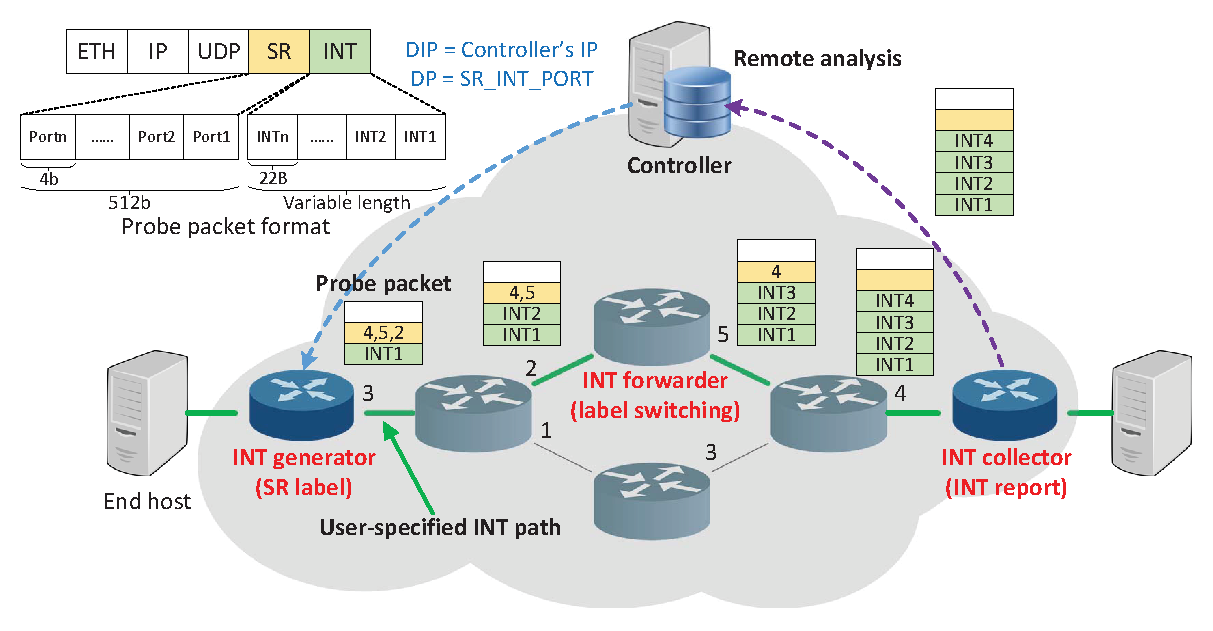
\epsfig{file=figure/demand_int1.eps, scale=0.435}
\vspace{-0.3cm}
\caption{Source routing-based path monitoring.}
\label{fig:demand_int1}
\vspace{-0.3cm}
\end{figure}

\textbf{Packet header format.}
In Fig.~\ref{fig:demand_int1}, we use a UDP packet to carry the SR-INT payload. To inform the packet parser that it is an SR-INT probe, the destination port (DP) number is set to ``SR\_INT\_PORT''. Above the UDP header, we reserve 512-bit for the SR label stack. We allocate 4-bit for each SR label to denote the router output port ID thus can maximally support 16 output ports for each router. Above the \emph{fixed-length} SR label stack, we allocate a \emph{variable-length} INT label stack. Each INT label occupies 22B containing the information such as device ID, ingress/egress port, egress queue depth. Since P4 currently does not well support parsing double variable-length stacks in the packet header, we statically allocate the SR label stack and use the right shift operation (``$\gg$'') to perform the ``stack pop'' behavior. The destination IP (DIP) address of the probe packet is set using controller's IP to guarantee that the probe packet will finally be forwarded to the controller for further analysis. Notice that although we design a customized header format for the probe packets, the network devices can still correctly forward these packets given \emph{protocol-independent forwarding}~\cite{bosshart2014p4} is supported.

\textbf{Forwarding behaviors.}
In the SR-based telemetry architecture, we propose three types of logic routers with different functionalities: the \emph{INT generator}, the \emph{INT forwarder} and the \emph{INT collector}. A physical device can simultaneously act as an INT generator and an INT collector. In other words, a physical device can be at the end of one monitoring path while at the start of another monitoring path at the same time.

The \emph{INT generator} is responsible for spawning the SR-INT probe packets at the first hop of the monitoring path. Since packet generation directly from the data plane is currently undefined by the P4 language, we consider a workaround to periodically generate ``empty'' probes from the outside by either the router/switch CPU or a server attached to the network device. When the probe arrives at the data plane, the INT generator will rewrite its packet header to add the SR label stack and its local INT information using \texttt{header.setValid()} and then forward the packet. Specifically, the INT generator will push the output port IDs into the SR label stack in the packet header. The sequence of the output port IDs (\ie, how to forward the packet across the network) is predetermined at the controller via centralized route calculation. 

The \emph{INT forwarder} performs packet forwarding of either the SR-INT probes or the ordinary traffic, according to the DP number of the incoming traffic. If the DP is ``SR\_INT\_PORT'', the INT forwarder will perform label switching (similar with MPLS) and forward the packet only according to the output port ID popped from the SR label stack (the DIP is no longer used in this case). The SR label is popped once at a router by right shifting the SR header by 4 bits at each hop. Besides, the INT forwarder will also push its local INT information into the INT label stack before forwarding the probe. 

At the last hop of the monitoring path, since the DIP is filled with controller's IP address, the \emph{INT collector} will finally forward the probe packet to the controller for further analysis.

\subsection{INT Path Planning for Graph Coverage (Policy)}
\label{subsec:policy}

Based on the SR-based telemetry mechanism, we can accurately control each probing path thus can develop diverse INT path planning algorithms for \emph{non-overlapped} INT path generation that covers the \emph{entire} network graph. Here, we first propose a simple algorithm based on \emph{depth-first search} (DFS), followed by a more sophisticated one based on \emph{Euler trail} which generates the \emph{optimal} result.

When traversing a tree or a graph, DFS starts at the root and explores as far as possible along each branch before backtracking. The basic idea of the DFS-based path planning algorithm is to consecutively add the visited vertices into the current path before backtracking; if we have nowhere to go and have to backtrack, we just create a new path and add the \emph{fork} vertex (the first vertex along the backtracking path that has unvisited edges) as the first node in the new path. After all the vertices are visited in the DFS order, we can extract multiple non-overlapped paths covering the entire graph.



Fig.~\ref{fig:dfs} shows a \emph{recursive} version of the DFS-based path planning algorithm. For each visited vertex, we will choose one of its unvisited edges for depth-first traversal (line 6-7 in Fig.~\ref{fig:dfs}). If we have chosen an unvisited edge, we will mark it as visited (line 8-9). We will explore as far as possible and add the visited vertices into the current INT path before backtracking occurs (line 17). On backtracking, we will create a new path from the fork vertex as the current path (line 12). In Fig.~\ref{fig:dfs}, we use the technique of recursion (line 19) to perform backtracking and leverage an additional \emph{flag} to locate the fork vertex during recursion. When a backtracking occurs during DFS, the current function call will return with \emph{true} (line 22) as its return value (which will be assigned to the bool variable \emph{flag} in its caller function in line 19). When the \emph{flag} is \emph{true} (line 10) and there is at least one unvisited edge (line 7), the currently visited vertex can be identified as a fork vertex (line 12-13) according to the previous definition. The recursion will finally halt when all the edges are visited. Besides, the first vertex $v_0$ of the depth-first traversal should be specially treated as a boundary case (line 1-3) and we have to invoke PathPlan($v_0$, \emph{true}) to start the algorithm. The run-time complexity of the algorithm is $O(V^2)$, similar with the classic DFS, if the graph is implemented with an adjacency matrix.

\begin{figure}
\centering
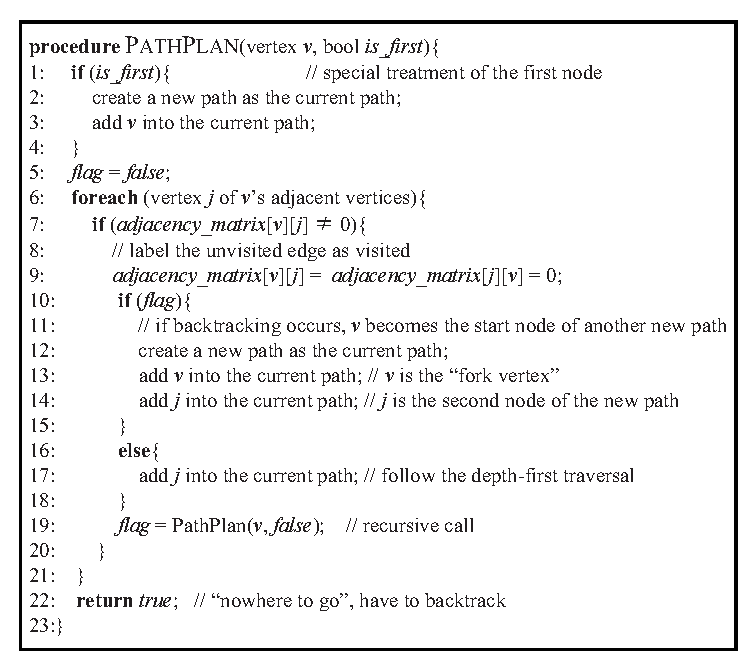
\epsfig{file=figure/algorithm.eps, scale=0.71}
\vspace{-0.2cm}
\caption{DFS-based INT path planning algorithm (a recursive version).}
\label{fig:dfs}
\vspace{-0.2cm}
\end{figure}

Fig.~\ref{fig:graph} shows an algorithm example on a network graph of five devices. After PathPlan($v_0$, \emph{true}) is invoked, $v_0$ is pushed into the call stack, path1 = \{$v_0$, $v_1$\} and the edge between $v_0$ and $v_1$ is marked as visited. The path1 expands as more and more vertices are visited in the DFS order. When path1 expands to \{$v_0$, $v_1$, $v_2$, $v_3$, $v_1$\}, we have nowhere to go and have to backtrack. At this time, we pop $v_1$ from the stack and return to $v_3$, which has an unvisited edge to $v_4$ (notice that the call stack push/pop operations are implicitly performed during recursion). Then, we identify $v_3$ as the \emph{fork} vertex because it is the first vertex along the backtracking path that has unvisited edges. Based on $v_3$, we create a new path as path2 = \{$v_3$, $v_4$\}. When path2 expands to \{$v_3$, $v_4$, $v_2$\}, we have again nowhere to go and have to backtrack. But at this time, although we check all the vertices popped from the call stack, we still cannot find any fork vertex. The recursion halts when the call stack finally becomes empty. At last, we extract two non-overlapped INT paths (\ie, path1 and path2).


\begin{figure*}[t]
    \centering
    \begin{minipage}[b]{0.345\textwidth}
        \centering
        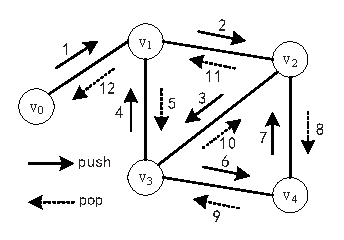
\includegraphics[width=0.75\textwidth]{figure/graph.eps} 
        \vspace{-0.2cm}
        \caption{Depth-first graph traversal.}\label{fig:graph}
    \end{minipage}
    % \hfill
    \hspace{0.0in}
    \begin{minipage}[b]{0.64\textwidth}
        \centering
        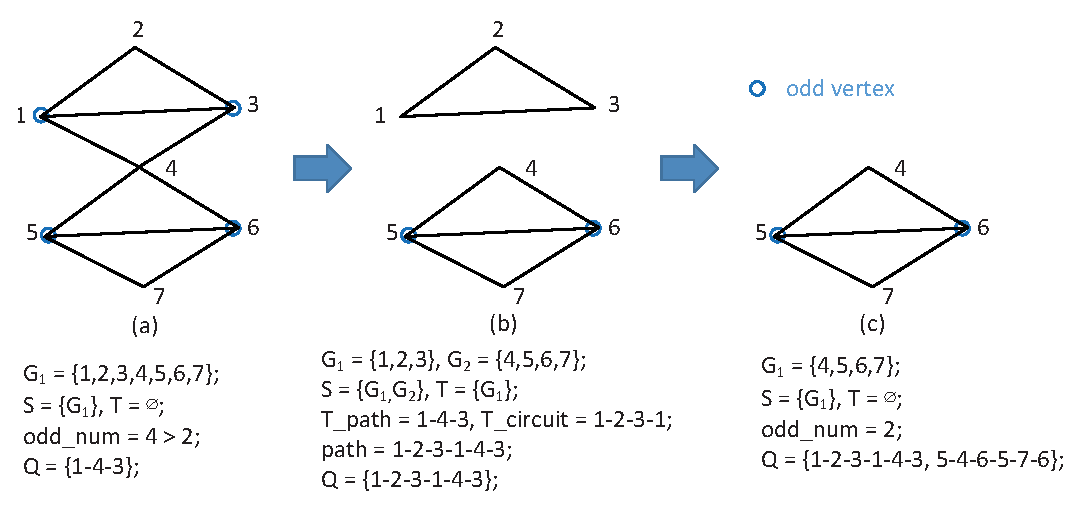
\includegraphics[width=0.78\textwidth]{figure/euler.eps}
        \vspace{-0.2cm}
        \caption{Path extraction process of the Euler trail-based algorithm.}\label{fig:euler}
    \end{minipage}
    \vspace{-0.45cm}
\end{figure*}











\section{Optimal Path Planning Policy}
\label{sec:algorithm}

\subsection{Properties of Euler Trail}

Although the DFS-based approach is time-efficient, it has \emph{no} guarantee to minimize the number of generated paths, which will increase the telemetry overhead, especially the telemetry workload at the centralized controller (as mentioned in \S\ref{subsec:challenge}). Besides, it exerts no optimization on the balanced path generation. Here, we propose an optimal path planning algorithm taking advantage of the mathematical properties of the Euler trail/circuit. In graph theory, a trail is a walk in a graph (\eg, $v_0$, $e_1$, $v_1$, $e_2$, ..., $v_k$) without repeated edges and an Euler trail is a trail which visits every edge exactly once. Similarly, an Euler circuit is a special Euler trail which starts and ends on the same vertex. To clarify the important theorems of the Euler trail/circuit, we give the definition of \emph{odd vertex} first. An odd vertex is a vertex who has an odd degree (\eg, vertex 1, 3, 5, 6 in Fig.~\ref{fig:euler}(a)). The following four theorems are well proved in graph theory: (1) a connected graph with \emph{no} odd vertex has an Euler circuit; (2) a connected graph with only \emph{one} odd vertex does not exist; (3) a connected graph with \emph{two} odd vertices has an Euler trail starts from one odd vertex and ends at the other one; (4) a connected graph with \emph{2k} odd vertices contains at least $k$ distinct trails which, together, traverse all edges of the graph exactly once~\cite{bondy1976graph}. The proposed optimal algorithm heavily relies on the above theorems.

\subsection{Algorithm Description}

In fact, the above properties (especially theorem (4)) give the \emph{theoretical} value of the minimum non-overlapped path number for covering a given graph. \emph{To achieve the theoretical minimum, each extracted path from a graph should starts from an odd vertex and ends at another odd vertex.} In other words, removing one such path from a graph will eliminate a pair of odd vertices of that graph. According to the above observation, we devise an Euler-trail based algorithm to iteratively extract a path between a pair of odd vertices until all the vertices are extracted from the graph (\ie, the degree of every vertex becomes zero). For a given graph with $2k$ odd vertices, our algorithm will generate $k$ non-overlapped paths (the theoretical minimum) to cover all edges of the graph. 



Although the algorithm sounds rather straightforward as an iterative path extraction process, \emph{the devil lies in the detail} of dealing with multiple boundary cases. To be more specific, the devil lies in the possibility that an extracted path can split one connected graph into multiple subgraphs, which definitely complicates the iterative path extraction process. For example, from Fig.~\ref{fig:euler}(a) to Fig.~\ref{fig:euler}(b) after the extraction of path 1-4-3, the connected graph is split into two subgraphs. Besides, the algorithm also need deal with (sub)graphs with no odd vertex (\eg, subgraph \{1,2,3\} in Fig.~\ref{fig:euler}(b)). We put the pseudocode of the optimal algorithm in Fig.~\ref{fig:algorithm2} and explain it in detail. 

\begin{figure}
\centering
\epsfig{file=figure/algorithm2.eps, scale=0.64}
\vspace{-0.35cm}
\caption{Euler trail-based path planning algorithm.}
\label{fig:algorithm2}
\vspace{-0.44cm}
\end{figure} 

Actually, without considering the complexity of graph split, for a given connected graph, there are mainly three different cases for path extraction. If the graph contains two odd vertices, we just find an Euler trail between the two odd vertices as the path to be extracted. If the graph contains more than two odd vertices, we should extract an Euler trail between any pair of odd vertices. If the graph does not contain any odd vertex, we can extract an Euler circuit from the graph, which traverses every vertex of the graph.

Specifically, we use $G$ to represent the graph set, which is initialized to be one connected graph and will contain one connected graph or multiple subgraphs caused by path extraction. We use $Q$ to represent the path set which is initialized as an empty set and will finally contain the generated non-overlapped INT paths. We use $G-p$ to represent extracting a path $p$ from the graph set $G$ which will possibly further split the graph(s) into more subgraphs. First, we consider a simple case that the algorithm input contains only one connected graph. If the graph has no odd vertex, an Euler circuit can be found with the Hierholzer's algorithm~\cite{hierholzer1873moglichkeit} and inserted into $Q$ (as implemented in line 17-19 in Fig.~\ref{fig:algorithm2}). Here, the Hierholzer's algorithm is an algorithm for finding Euler trails/circuits with a run-time complexity of $O(E)$~\cite{fleischner1991x}, which is more efficient than the famous Fleury's algorithm~\cite{fleury1883deux}. If the graph has two odd vertices, an Euler trail can also be found with the Hierholzer's algorithm and inserted into $Q$ (line 25-26, line 31-32). If the graph has more than two odd vertices, we just randomly choose two odd vertices and find a path (\eg, with the Dijkstra's algorithm or any other algorithms) to connect the pair of odd vertices, then we insert the path into $Q$ (line 28-29, line 31-32). Notice that each time we extract a path from $G$ and insert it into $Q$, the graph(s) in $G$ may be broken into multiple disconnected subgraphs. Next, we discuss how to handle this boundary case in detail.

We use $S$ to save the disconnected subgraphs split from $G$ via DFS traversal (line 2). Then, we select graphs with \emph{no} odd vertex from $S$ and save them into $T$ (line 3). For each graph in set $T$, we can generate an Euler circuit $T\_circuit$ for its full edge coverage (line 9 and line 17). However, $T\_circuit$ is \emph{inadequate} to become a final INT path, since if the initial graph has $2k$ odd vertices ($k>0$), all the $k$ INT paths should connect $k$ pairs of odd vertices. By contrast, $T\_circuit$ does not contain any odd vertex. For this situation, there is only one possibility that $T\_circuit$ must be an integral part of a final INT path. In other words, $T\_circuit$ should be successfully connected to one calculated Euler trail to form a longer Euler trail. Here, we give a simple proof of the above hypothesis that $T\_circuit$ is an integral part of a final INT path.

\textbf{Proposition 1.}
In the Euler trail-based path planning algorithm (Fig.~\ref{fig:algorithm2}), if $T \neq \emptyset$ and $Q \neq \emptyset$ (\ie, there is at least one (sub)graph $g$ that does not contain odd vertex and there has been at least one calculated Euler trail in $Q$), $T\_circuit$ (the Euler circuit of $g$) should be successfully connected to one of the calculated Euler trails in $Q$ to form a longer Euler trail.

\begin{proof}
We construct a simple proof by \emph{contradiction}. Suppose $T\_circuit$ cannot connect to any of the Euler trails in $Q$. Then, there must be two possibilities: (1) $g$ itself is the initial graph $G$; (2) $g$ is once a part of the initial graph $G$. For case (1), if $g$ is the initial graph, then $Q$ must be an empty set, which contradicts with the premise that $Q \neq \emptyset$. For case (2), if $g$ is once a part of the initial graph $G$, then $g$ must have at least one common vertex $v$ with graph $G - T\_circuit$. If $T\_circuit$ cannot connect to any of the Euler trails in $Q$, then $v$ does not belong to any of the Euler trails in $Q$. However, according to the algorithm in Fig.~\ref{fig:algorithm2}, graph split occurs only after the extraction of Euler trails. If $v$ is not on the Euler trails, then $g$ must be still connected with $G - T\_circuit$ on $v$, which contradicts with the premise that $g$ is a separate subgraph.
\end{proof}

% 如果T_circuit无法连接Q中的欧拉路径,那么顶点v也无法连接Q中的欧拉路径。同时,根据我们的算法,图只能被产生的欧拉路径进行分割,如果v没有在欧拉路径上,那么T_circuit在算法运行完成后仍然和G-T_circuit相连,这就和T_circuit是一个独立的图相矛盾。


If $T \neq \emptyset$ and $Q \neq \emptyset$, we search the current $Q$ to find a path $T\_path$ having at least a same vertex with $T\_circuit$ (line 7). Then, we connect $T\_circuit$ with $T\_path$ to create a longer new path via \texttt{pathPaste()} (line 10) and replace the original $T\_path$ with the new path in $Q$ (line 8, 11).

In summary, the algorithm iteratively extracts paths connecting two odd vertices or pastes Euler circuits to the previous extracted paths to form the final INT paths. The algorithm halts if all the vertices are extracted from the graph (\ie, $G = \emptyset$).





\subsection{Case Study}
Fig.~\ref{fig:euler} exemplifies a path extraction process of the Euler trail-based algorithm. At the start, there is only one graph $G_1$ \{1,2,3,4,5,6,7\} with 4 odd vertices. Since the number of the odd vertices is larger than 2 (line 28), we randomly choose two odd vertices (1 and 3), extract a path 1-4-3 from $G_1$ and insert the path into $Q$ (Fig.~\ref{fig:euler}(a)). The above path extraction behavior will split the original $G_1$ into two subgraphs $G_1$ \{1,2,3\} and $G_2$ \{4,5,6,7\}. Since $G_1$ has no odd vertex and $Q \neq \emptyset$ (line 4-5), we paste the path 1-4-3 in $Q$ with the Euler circuit 1-2-3-1 generated from $G_1$ to create a new path 1-2-3-1-4-3. The new path will replace the original path 1-4-3 in $Q$ (Fig.~\ref{fig:euler}(b)). After the path paste, there is only one graph $G_1$ \{4,5,6,7\} with 2 odd vertices (line 25). We use the Hierholzer's algorithm to find its Euler trail 5-4-6-5-7-6 as the second INT path in $Q$ (Fig.~\ref{fig:euler}(c)). The algorithm halts since all the paths are extracted.

\subsection{Run-Time Complexity Analysis}
\label{subsec:theory}

The complexity of the above algorithm is analyzed. Since the algorithm is quite sophisticated, here, we strive to give an \emph{upper bound} for its run-time complexity as follows.

\textbf{Assumption.}
The input of the algorithm is an undirected connected graph $G=(V,E)$ with $2k$ odd vertices ($k = 0,1,2,...$). The graph is implemented via the adjacency list. We only consider the most time-consuming subprocedures in the algorithm, namely, (a) DFS for graph split (line 2), (b) \texttt{eulerCircuit()} and \texttt{eulerTrail()}, both using the Hierholzer's algorithm (line 9, 17, 26), (c) \texttt{randomTrail()} using the Dijkstra's algorithm (line 29). The time cost $T$ of the three subprocedures can be represented as $T(DFS(V,E)) = (E+V)t_0$, $T(Euler(V,E)) = Et_0$, $T(Dij(V,E)) = Et_0$, all based on their fastest implementation~\cite{cormen2009introduction, hierholzer1873moglichkeit, thorup1999undirected}, where $t_0$ is the one memory access time of the adjacency list.

\textbf{Complexity analysis case by case.}

1. If $k = 0,1$, $G$ has one Euler circuit or one Euler trail. In this case, DFS will be performed to check the graph connectivity, and \texttt{eulerCircuit()} or \texttt{eulerTrail()} will be performed to extract the path. Hence, the time cost can be derived as $T = T(DFS(V,E)) + T(Euler(V,E))$.

2. If $k > 1$, $G$ must have at least 4 odd vertices.

2.1. For the first iteration of the algorithm, DFS will be performed to check the connectivity, then, \texttt{randomTrail()} will be performed to extract one shortest path between 2 odd vertices. The time cost $T_1 = T(DFS(V,E)) + T(Dij(V,E))$.

2.2. For the next iteration, after the path extraction, the graph $G = (V, E)$ becomes $G' = (v, e)$. Then, we use DFS to check its connectivity. The path extraction may split $G'$ into subgraphs. We use $S$ to represent the subgraph set. For this step, the time cost $T_2 = T(DFS(v,e))$.

2.3. Set $S$ can further be partitioned into two subsets with one subset $T$ containing subgraphs \emph{without} odd vertices and the other subset $S-T$ containing subgraphs \emph{with} odd vertices. We define $T = \{g_x'|g_x'=(v_x', e_x'), x = 1,2,...\}$, $S-T = \{g_y''|g_y''=(v_y'',e_y''), y=1,2,...\}$. We have $\sum_{x}v_x' + \sum_{y}v_y'' = v$, $\sum_{x}e_x' + \sum_{y}e_y'' = e$.

2.4. For each subgraph $g_x'$ in subset $T$, we will perform \texttt{eulerCircuit()} and \texttt{pathPaste()}. Since \texttt{eulerCircuit()} is much more time-consuming, we only consider its time cost as $T_3 = \sum_xT(Euler(v_x',e_x'))$.

2.5. For each subgraph $g_y''$ in subset $S-T$, if $g_y''$ has exactly 2 odd vertices, we will perform \texttt{eulerTrail()}; if $g_y''$ has more than 2 odd vertices, we will perform \texttt{randomTrail()}. Given we have $y_1$ subgraphs with exactly 2 odd vertices and $y_2$ subgraphs with more than 2 odd vertices, the time cost of this step can be derived as $T_4 = \sum_{y_1}T(Euler(v_{y_1}'',e_{y_1}'')) + \sum_{y_2}T(Dij(v_{y_2}'',e_{y_2}''))$.

2.6. The iteration will go back to 2.2. until $G$ becomes $\emptyset$.

Given the algorithm is iterated for $m$ times, the total time cost can be derived as $T = T_1 + \sum_{i}^{m-1}(T_{2i} + T_{3i} + T_{4i})$, where $i$ stands for the ($i+1$)th iteration ($0 < i < m$).


\textbf{Upper bound derivation.}
The complexity of the algorithm lies in that the number of subgraphs in $T$ or $S-T$ for each iteration as well as the algorithm execution path cannot be predetermined. Here, we derive an \emph{upper bound} for algorithm's run-time complexity considering its \emph{worst-case execution path}. 

First, we try to solve $T_3 = \sum_xT(Euler(v_x',e_x'))$. Considering $T(Euler(v,e)) = et_0$, given $e' = \sum_{x}e_x'$, we have $T_3 = \sum_xT(Euler(v_x',e_x')) = \sum_{x}e_x't_0 = e't_0$.

Then, we try to solve $T_4$. According to our algorithm, the number of odd vertices of each subgraph in $S-T$ will be decreased by 2 in each iteration. Hence, the total number of decreased odd vertices in each iteration will be $2(y_1+y_2)$. According to the assumption, the total number of decreased odd vertices in $m$ iterations is $2k$. In the worst case, the iteration times $m$ should be \emph{maximized} while the number of decreased odd vertices in each iteration should be \emph{minimized}. In this case, $m = k$, $y_1 = 0, y_2 = 1$ for the first k-1 iterations and $y_1 = 1, y_2 = 0$ for the $k$th iteration. That is to say, the total number of decreased odd vertices in each iteration will be limited to 2. In this case, we have $T_{4i} = T(Dij(v_i'',e_i''))$ ($i = 1,2,...,k-2$) and $T_{4i} = T(Euler(v_i'',e_i''))$ ($i = k-1$).

According to the above analysis, we have $T = T_1 + \sum_{i}^{m-1}(T_{2i} + T_{3i} + T_{4i}) \le T(DFS(V,E)) + T(Dij(V,E)) + \sum_{i=1}^{k-2}(T(DFS(v_i,e_i)) + e_i't_0 + T(Dij(v_i'', e_i''))) + T(DFS(v_{k-1}, e_{k-1})) + e_{k-1}'t_0 + T(Euler(v_{k-1}'',e_{k-1}''))$, where $e_i$ is the edge set of $G' = (v,e)$,  $e_i'$ is the edge set of the subgraph subset $T$ and $e_i''$ is the edge set of the subgraph subset $S-T$, all in the ($i+1$)th iteration. Similarly, $v_i$ and $v_i''$ are the vertex sets of $G'$ and $S-T$, respectively. Apparently, we have $e_i = e_i' + e_i''$ and $v_i = v_i' + v_i''$.

According to the worst-case assumption, there is at least one subgraph in $T$ and there is only one subgraph in $S-T$ for each iteration. Therefore, $G_i'$ for the ($i+1$)th iteration is generated from $G_{i-1}'$ by removing all the subgraphs from $T$ and one shortest path from $S-T$. Using the above \emph{recurrence relation}, we can further derive algorithm's run-time complexity $T$. 

Actually, the minimal subgraph without odd vertices is the \emph{triangle}, which has 3 vertices and 3 edges, while the minimal shortest path is the \emph{line segment} which has 2 (odd) vertices and 1 edge. Therefore we have $e_i' \ge 3$, $v_i' \ge 3$, $e_i'' \ge 1$, $v_i'' \ge 2$, $e_i \le e_{i-1}-3-1$, $v_i \le v_{i-1} -3$. By plugging the initial values $e_0 = E, v_0 = V$ into the above relations, we have $e_i \le E-4i$, $v_i \le V - 3i$. Based on above relations, we can further derive

$e_i' = e_i - e_i'' \le e_i - 1 \le E-4i-1$,

$v_i' = v_i - v_i'' \le v_i - 2 \le V-3i-2$,

$e_i'' = e_i - e_i' \le e_i - 3 \le E-4i-3$,

$v_i'' = v_i - v_i' \le v_i - 3 \le V-3i-3$.

By plugging the above relations into the expression of $T$, we derive an upper bound for the run-time complexity as

$T \le (E+V)t_0 + Et_0 + \sum_{i=1}^{k-2}((e_i + v_i)t_0 + e_i't_0 + e_i''t_0) + (e_{k-1} + v_{k-1})t_0 + e_{k-1}'t_0 + e_{k-1}''t_0 \le (2E+V)t_0 + \sum_{i=1}^{k-1}(e_i + v_i + e_i' + e_i'')t_0 \le (2E+V)t_0 + \sum_{i=1}^{k-1}(E-4i + V-3i + E -4i -1 +E -4i -3)t_0 \le (3kE + kV - \frac{15}{2}k^2 -E + \frac{7}{2}k + 4)t_0$.

Therefore, one upper bound for algorithm's run-time complexity can be represented as $O(k(3E + V -\frac{15}{2}k))$.








\subsection{Heuristic for Balanced Path Generation}
\label{subsec:balance}

As mentioned in \S\ref{subsec:challenge}, balanced path generation is preferable to facilitate synchronized multi-path monitoring. However, our algorithm does not explicitly optimize for this particular purpose. Here, we propose a simple \emph{heuristic} for more balanced path generation based on the original algorithm. 

According to our extensive debugging of the original algorithm, we find that the path connecting two odd vertices generated by function \texttt{eulerTrail()} in line 26 is often \emph{too short} compared with the average length of the Euler trails. The reason lies in that in our implementation of \texttt{eulerTrail()}, we return the shortest path between two \emph{randomly} selected odd vertices with the Dijkstra's algorithm. If the path cannot properly paste to an Euler circuit afterwards to form a longer Euler trail, the final INT paths will be less balanced.

To address this issue, we propose a heuristic for more balanced path generation simply by rewriting the function \texttt{eulerTrail()}. Instead of returning the shortest path between two randomly selected odd vertices, we calculate all the shortest paths between any given pair of odd vertices and return the \emph{longest} path from all these shortest paths. Such a tweak greatly reduces the length variance of final INT paths.

However, on each extraction of an Euler trail, we have to recalculate $C_n^2$ ($n$ is the number of odd vertices) shortest paths due to the graph update, which is time-consuming. Here, we propose a technique to further minimize the computation cost. Actually, in our algorithm, we always remove edges from the graph during path extraction while never add edges into the graph. Hence, if the calculated shortest path has no intersection with the extracted Euler trail, the shortest path need not be recalculated. By checking the intersection of the extracted path and the shortest paths, we can update the shortest paths \emph{on demand} and eliminate unnecessary computation cost.







\section{Evaluation}
\label{sec:evaluation}

\subsection{Experimental Setting}

We build a network prototype to demonstrate the proposed \emph{INT-path}. The hardware is with i7-6700K CPU and 16GB memory, running Ubuntu 16.04 OS. The prototype is implemented using Mininet and consists of 1 controller, 18 switches and 12 end hosts. Specifically, we adopt the P4 software switch (\ie, bmv2~\cite{bmv2}) to achieve the capability of protocol-independent header rewriting and forwarding of customized INT packets which contain additional source routing metadata. The controller speaks with bmv2 using Thrift. Each end host is responsible for generating 1kpps background UDP traffic with randomly changed destination addresses. The packet interval follows Poisson distribution. The end hosts also generate ``empty'' probes for P4 switches to further rewrite the header and create the SR-INT probes. The deployment locations of the INT generators/collectors as well as the source routing paths embedded in the SR-INT probes are precalculated by the Euler trail-based path planning algorithm. The default INT packet sending rate is set to 100pps. On receiving the INT packet, the controller will parse the packet header and write the telemetry data into a local database, where the global traffic status can be summarized and visualized. 



The two path planning algorithms (\ie, DFS and Euler) are implemented with Python. The efficiency of the algorithms are evaluated upon randomly generated graphs of difference sizes as well as two data center topologies (\ie, FatTree and LeafSpline). We evaluate the metrics such as generated INT path number, INT path length variance, telemetry overhead, algorithm execution time, impact of odd vertex number.


The entire system consists of 2464 lines of Python, 324 lines of P4, 191 lines of C and 16 lines of SQL, which is available at our git repository~\cite{git}.

Before diving into the analysis of experimental data, we first show some output results from INT-path to give the reviewers some intuitive feeling about our system. Fig.~\ref{fig:bitmap} shows the network-wide traffic status in one snapshot under varying traffic loads. The network-wide traffic status (here, queue depth) is ``encoded'' into a series of ``bitmap images'' in real time. By analyzing the ``bitmap images'', one can dig out insightful knowledge from the underlying network (\eg, from Fig.~\ref{fig:bitmap_high}, we can find that link(12, 11) is heavily congested). Such concise network status representation may further allow using advanced techniques for big network data analysis.

\begin{figure}[t]
\vspace{-0.0in}
\centering
\subfigure[Network is lightly loaded.]{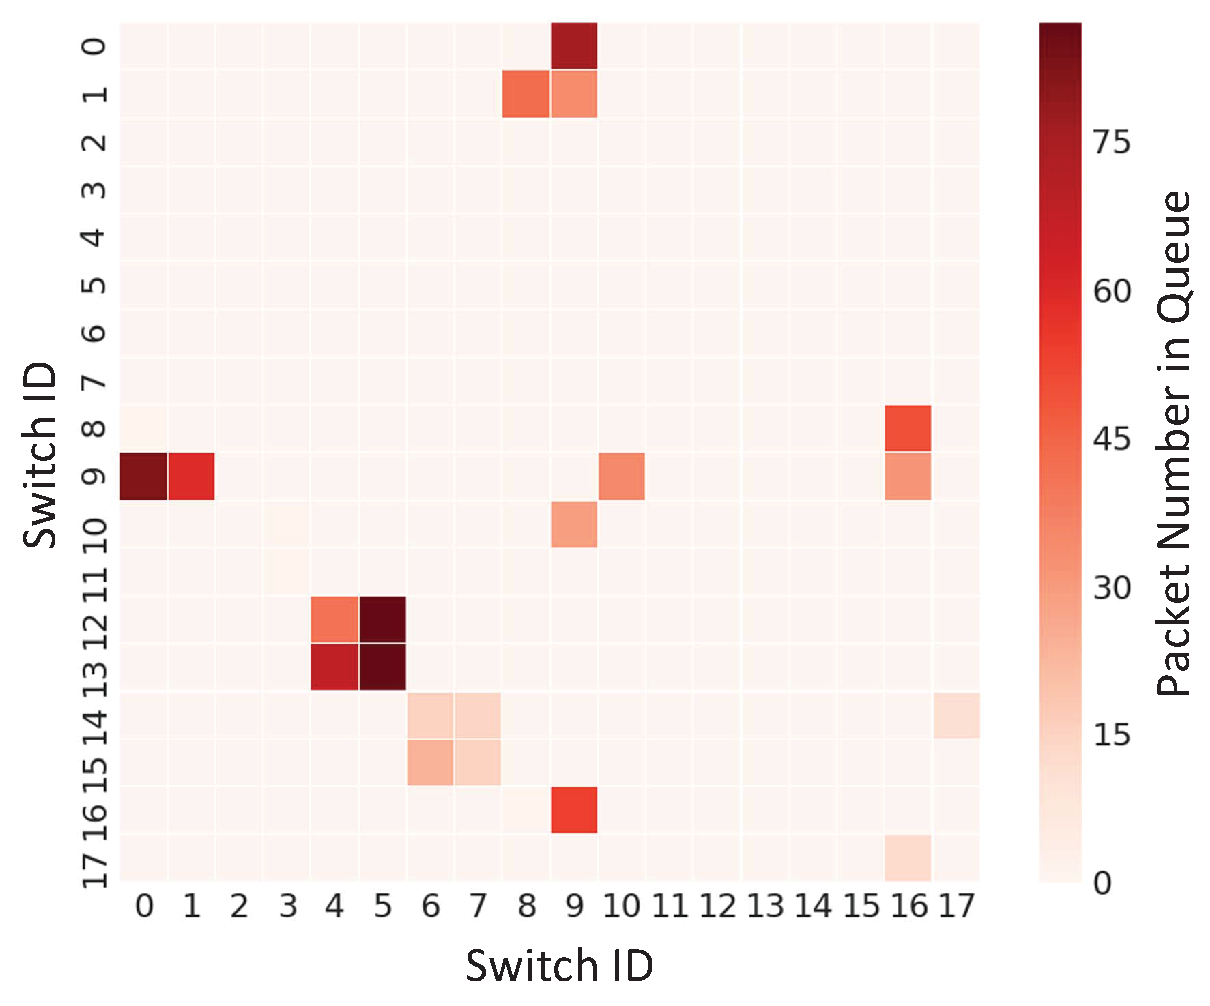
\includegraphics[width=0.22\textwidth]{figure/bitmap_low.eps}\label{fig:bitmap_low}}
\vspace{-0.1cm}
\subfigure[Network is heavily loaded.]{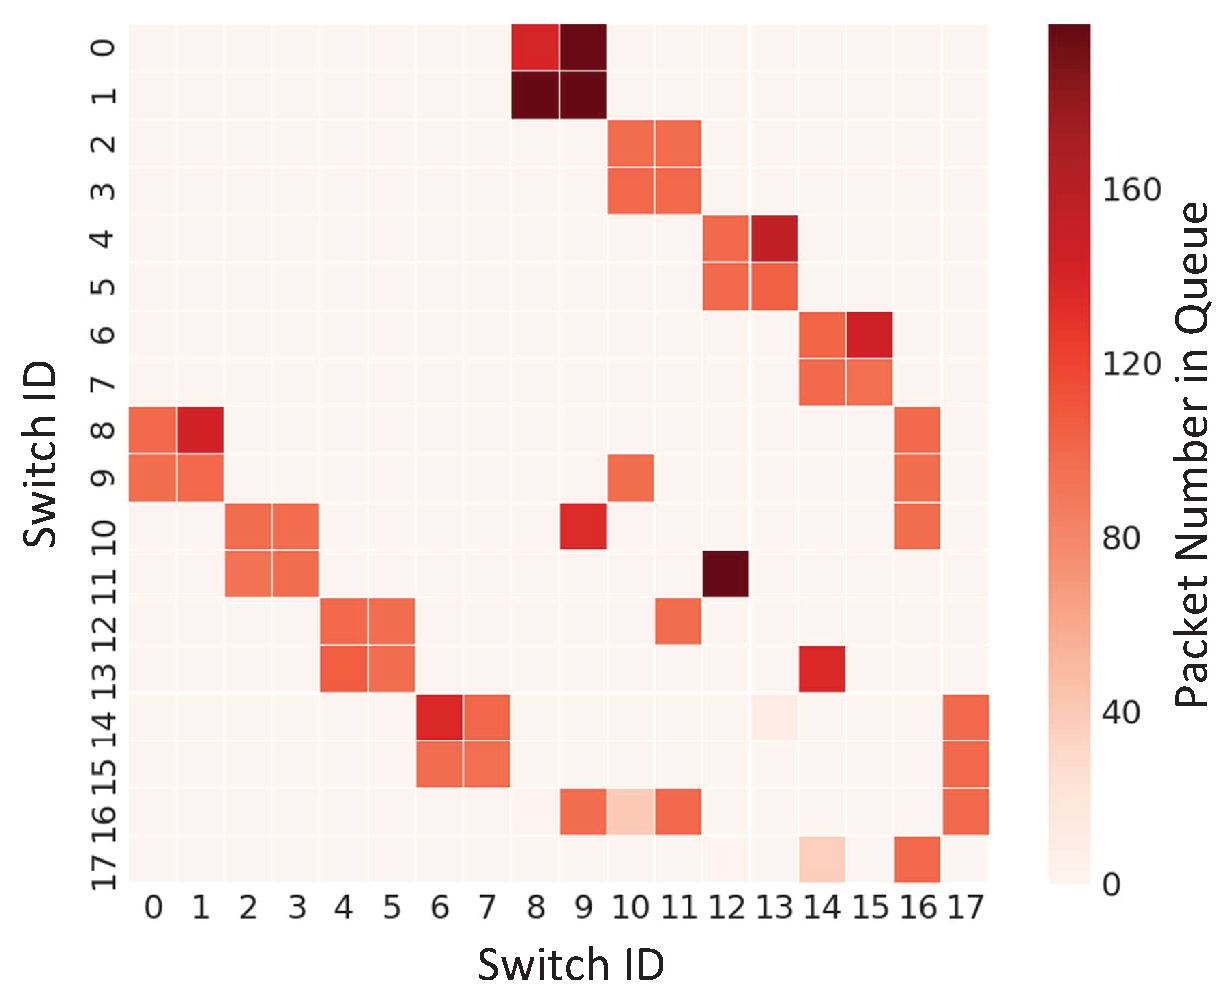
\includegraphics[width=0.22\textwidth]{figure/bitmap_high.eps}\label{fig:bitmap_high}}
\vspace{-0.1cm}
\caption{Network-wide traffic visibility as a series of ``bitmap images''.}
\label{fig:bitmap}
\vspace{-0.4cm}
\end{figure}

\subsection{Experimental Results}

\begin{figure*}[htbp]
	\vspace{-0.2cm}
\minipage{0.24\textwidth}
	\vspace{0.0cm} 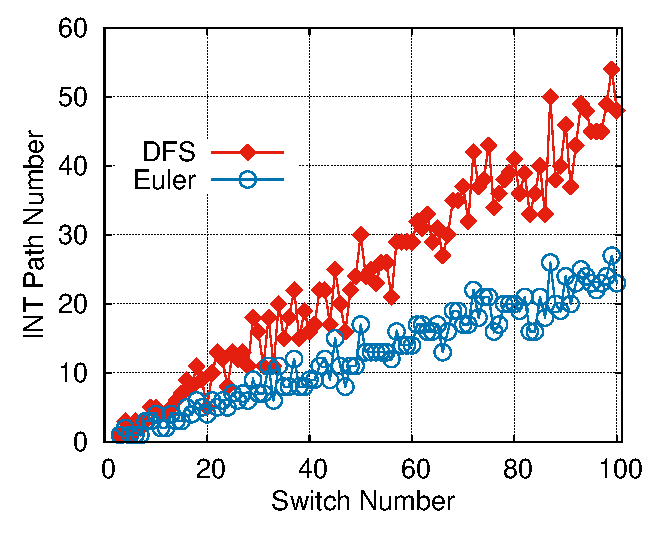
\includegraphics[width=\linewidth]{figure/path_num.eps}
	  \center
	  \vspace{-0.0cm}
	  \caption{Number of INT paths from DFS and Euler trail-based algorithms.}\label{fig:path_num}
	\endminipage\hfill
    	\minipage{0.24\textwidth}
					\vspace{-0.0cm} 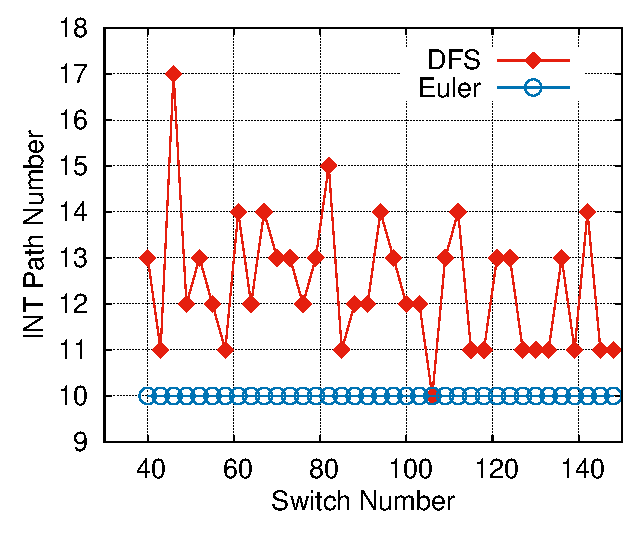
\includegraphics[width=\linewidth]{figure/fix_odd.eps}
					  \center
					  \vspace{0.0cm}
					  \caption{Number of INT paths generated under a fixed odd vertex number}\label{fig:fix_odd}
					\endminipage\hfill
	\minipage{0.24\textwidth}
                    \vspace{-0.0cm} 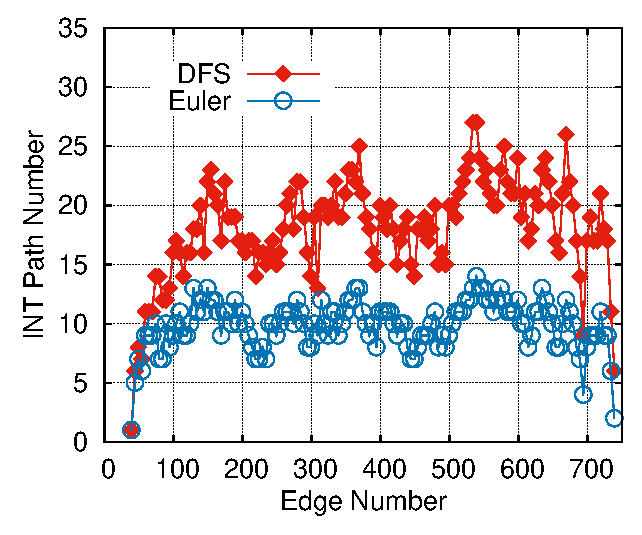
\includegraphics[width=\linewidth]{figure/fix_vertex.eps}
			  \center
			  \vspace{-0.0cm}
			  \caption{Number of INT paths generated under a fixed vertex number}\label{fig:fix_vertex}
			\endminipage\hfill
					\minipage{0.244\textwidth}
					\vspace{-0.0cm} 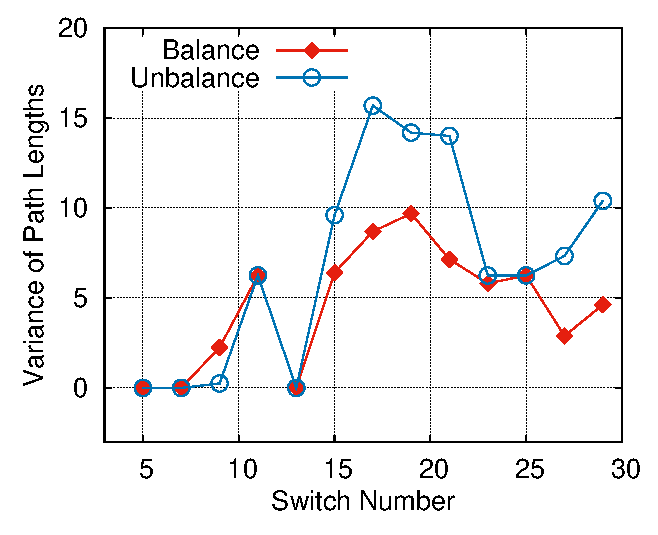
\includegraphics[width=\linewidth]{figure/balance.eps}
					  \center
					  \vspace{0.0cm}
					  \caption{Variance of path lengths with balanced and unbalanced algorithms.}\label{fig:balance}
					\endminipage
					 
\vspace{-0.3cm}
\end{figure*}


\begin{figure*}[htbp]
	\vspace{-0.0cm}
\minipage{0.24\textwidth}
	\vspace{0.0cm} 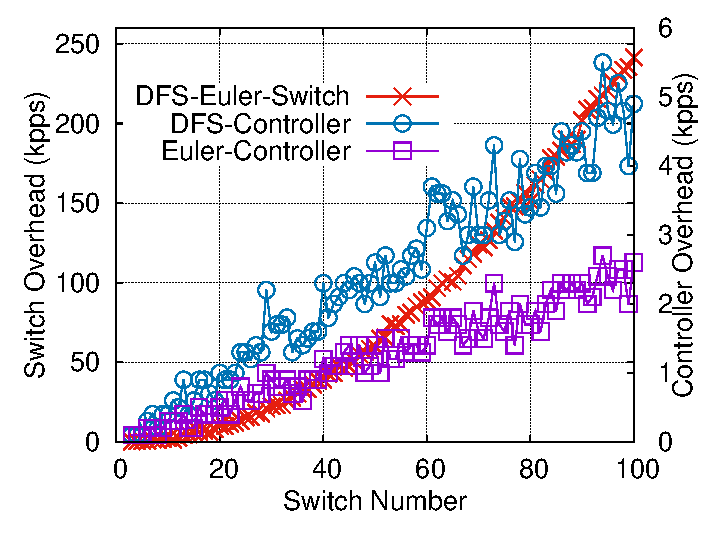
\includegraphics[width=\linewidth]{figure/overhead.eps}
	  \center
	  \vspace{-0.0cm}
	  \caption{Telemetry overhead of DFS and Euler on controller and data plane.}\label{fig:overhead}
	\endminipage\hfill
	\minipage{0.24\textwidth}
			\vspace{-0.0cm} 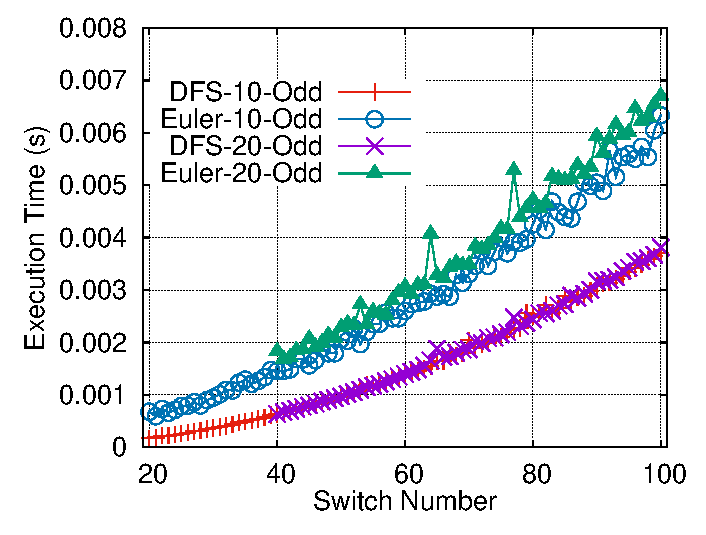
\includegraphics[width=\linewidth]{figure/runtime.eps}
			  \center
			  \vspace{-0.0cm}
			  \caption{Execution time of DFS and Euler upon a growing network size.}\label{fig:runtime}
			\endminipage\hfill
			\minipage{0.255\textwidth}
					\vspace{-0.0cm} 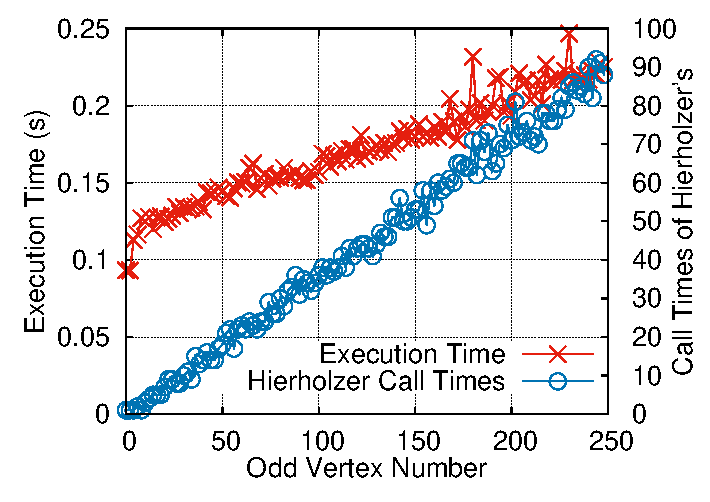
\includegraphics[width=\linewidth]{figure/odd.eps}
					  \center
					  \vspace{0.0cm}
					  \caption{Impact of odd vertex number on Euler's execution time (500 switches.)}\label{fig:odd}
					\endminipage\hfill
					\minipage{0.24\textwidth}
					\vspace{-0.0cm} 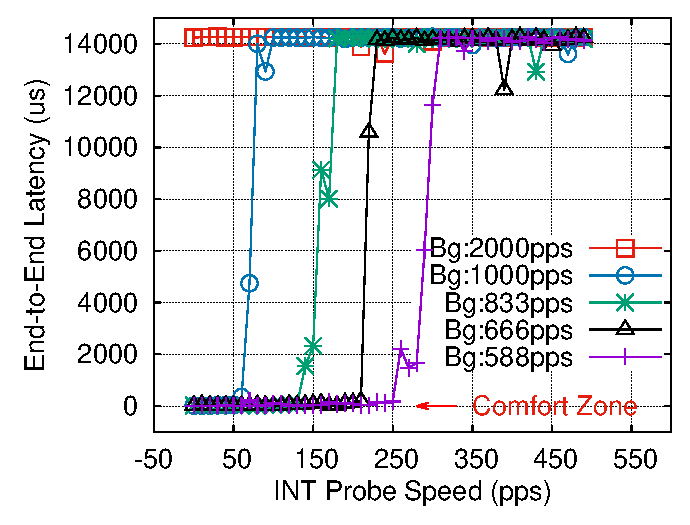
\includegraphics[width=\linewidth]{figure/impact.eps}
					  \center
					  \vspace{0.0cm}
					  \caption{Impact of telemetry granularity on system performance.}\label{fig:impact}
					\endminipage
					 
\vspace{-0.55cm}
\end{figure*}

\textbf{Number of generated INT path.}
Fig.~\ref{fig:path_num} shows the number of generated INT paths from DFS and Euler trail-based algorithms on randomly generated graphs. The path number of both DFS and Euler grow roughly linearly with the graph size while the Euler generates less INT paths than DFS under any fixed switch number. As we have mentioned, the number of paths generated from Euler is the theoretical minimum and only decided by the odd vertex number of the graph. In Fig.~\ref{fig:path_num}, since the graph is randomly created, Euler's path number grows together with the odd vertex number as the graph becomes larger. In Fig.~\ref{fig:fix_odd}, when we fix the number of odd vertices in a graph, the INT path number generated from Euler becomes a constant no matter what size the network grows into. In Fig~\ref{fig:fix_vertex}, when we fix the number of vertices to a constant (\eg, 39 in our experiment) and grow the network size by adding more edges, we can find that the path number generated from both DFS and Euler grow at the first and decline in the end. This is because adding more edges at the start makes the graph become more complex with more odd vertices while in the end, the graph finally becomes a complete graph without odd vertices (in a complete graph, every pair of distinct vertices is connected by a unique edge and each of the 39 vertices has 38 connected edges). Despite this, Euler still outperforms DFS to generate less INT paths in Fig~\ref{fig:fix_vertex}.

\textbf{Balanced vs unbalanced path generation.}
Fig~\ref{fig:balance} shows the variance of the path lengths generated from the original version of Euler and a later improved version considering path balance (\S\ref{subsec:balance}). We can figure out that by adding the heuristic for balanced path generation by rewriting \texttt{randomTrail()}, the variance of the path lengths becomes lower compared with the original Euler on randomly generated graphs.



\textbf{Telemetry overhead.}
Fig.~\ref{fig:overhead} shows the INT telemetry overhead of DFS and Euler trail-based algorithms on both the controller and the switches. The telemetry overhead on the controller is mainly caused by INT probe collection. The traffic volume of the probes forwarded to the controller is decided by the INT sending rate as well as the number of INT collectors, which is further decided by the number of INT paths generated by the algorithms. In Fig.~\ref{fig:overhead}, when the switch number is 100, DFS floods 5kpps probes to the controller while Euler only floods 2.5kpps due to the minimum generated path number. For the data plane, the telemetry overhead is measured as the total number of INT probes processed by switches per second. Since both DFS and Euler will traverse all edges of the graph, they have the same switch telemetry overhead. The switch telemetry overhead is only affected by the network size and the INT sampling granularity.

\textbf{Execution time of path planning algorithms.}
Fig.~\ref{fig:runtime} shows the execution time of DFS and Euler upon a growing network size. According to our exhaustive analysis of Euler's run-time complexity in \S\ref{subsec:theory}, Euler's execution time is larger than DFS's. Besides, Euler's execution time is more sensitive to the odd vertex number of the graph. In Fig.~\ref{fig:odd}, we find that the execution time of Euler trail-based algorithm grows roughly linearly with the odd vertex number. This result also validates our run-time complexity analysis that the subprocedures \texttt{randomTrail()}, \texttt{EulerTrail()} and \texttt{EulerCircuit()} are most frequently executed in our algorithm which are related with the odd vertex number.

\textbf{Impact of telemetry granularity.}
To achieve fine-grained network-wide telemetry, \ie, to obtain the precise real-time traffic dynamics in the network, the INT probe generation speed is expected to be as high as possible. However, this will not only lay heavy performance burden on the controller, but also occupy the limited link bandwidth, causing traffic congestion or even router buffer overflow. That is to say, there should be a limit of the telemetry granularity, constrained by controller's ability and link's capacity. Fig.~\ref{fig:impact} shows this extreme situation. In Fig.~\ref{fig:impact}, the x-axis is the INT probe generation speed at each end host and the y-axis is the end-to-end link latency along the probing path. We can figure out that when the INT probe generation speed grows, there is a sudden change of the end-to-end latency. This is because the buffer of the switches along the probing path become overflow at that time and start to drop packets. To make the experimental results more significant, we set a shallow buffer of 100 packets for each P4 switch and the buffer overflow occurs very soon. Besides, the background traffic rate also has an impact on the end-to-end latency of the probe packets. For INT-path deployment in real-world networks, we recommend to properly arrange the telemetry granularity into the ``comfort zone'' in Fig.~\ref{fig:impact}, considering the switch buffer size configuration and the background traffic rate.
%需要讲队列长度比较短,几百,一会儿就满了,导致最大时延比较恒定



\textbf{Network-wide telemetry in DC networks.}
In the previous sections, we discuss the performance of Euler trail-based algorithm on randomly generated graphs. Here, we investigate its performance in today's data center networks. Designing for better load balancing, classic data center network topologies are symmetric and have several multi-path topology patterns. Fig.~\ref{fig:dc} shows two classic DC network topologies: FatTree and LeafSpine. We find that the odd vertex number in both topologies are very predictable depending on the scale of the networks. For example, in FatTree, there are three layers of switch nodes, and the layer 1 and layer 3 do not have odd vertices no matter what the scale of the network. However, in layer 2, the number of the odd vertices regularly changes depending on the size of the network. LeafSpine shows the similar property. This property is very helpful when we design DC networks with In-band network-wide telemetry features. If the DC network topology has an even number of basic units (as shown in Fig~\ref{fig:dc}), at best, we can use one INT telemetry path to cover the entire network. If it has an odd number $\ie, k$ of units, we have to plan $k$ telemetry paths for the full network coverage. Fig.~\ref{fig:topo} shows the comparison between DFS and Euler on DC network topologies. We can find the symmetric topology of DC networks even makes DFS output predicable! However, Euler still outperforms DFS in either DC topology.

\begin{figure}
\centering
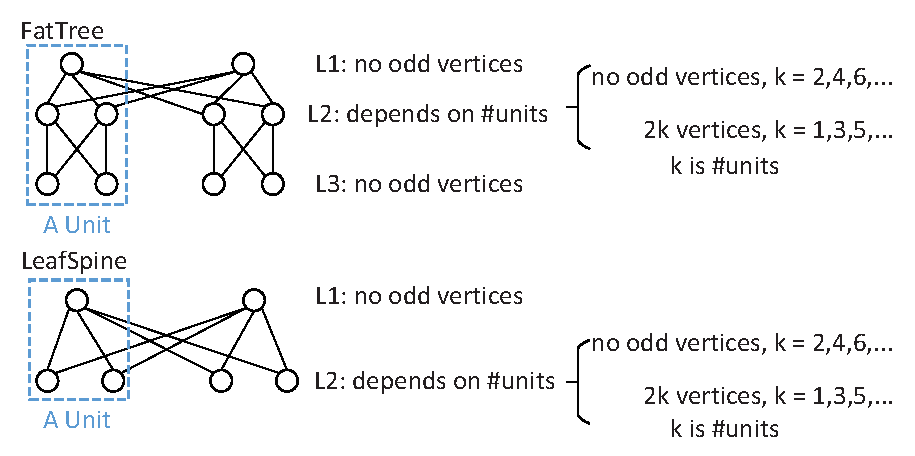
\epsfig{file=figure/dc.eps, scale=0.45}
\vspace{-0.3cm}
\caption{Two classic data center network topologies.}
\label{fig:dc}
\vspace{-0.4cm}
\end{figure}



\begin{figure}[t]
\vspace{-0.0in}
\centering
\subfigure[FatTree topology.]{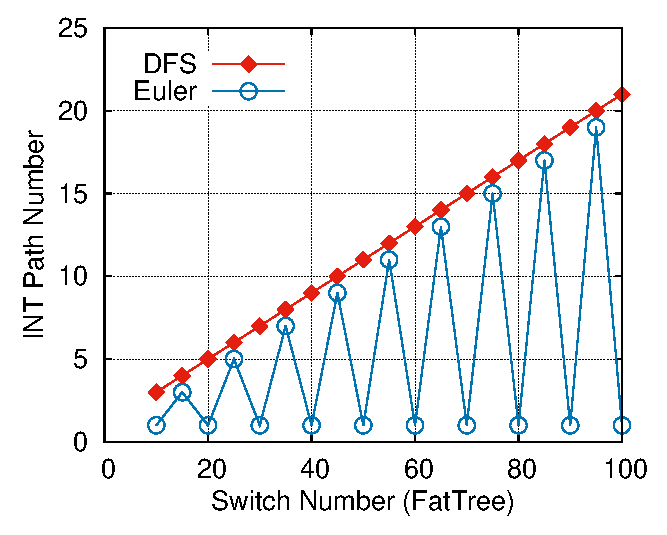
\includegraphics[width=0.23\textwidth]{figure/fat_tree.eps}\label{fig:fat_tree}}
\vspace{-0.15cm}
\subfigure[LeafSpine topology.]{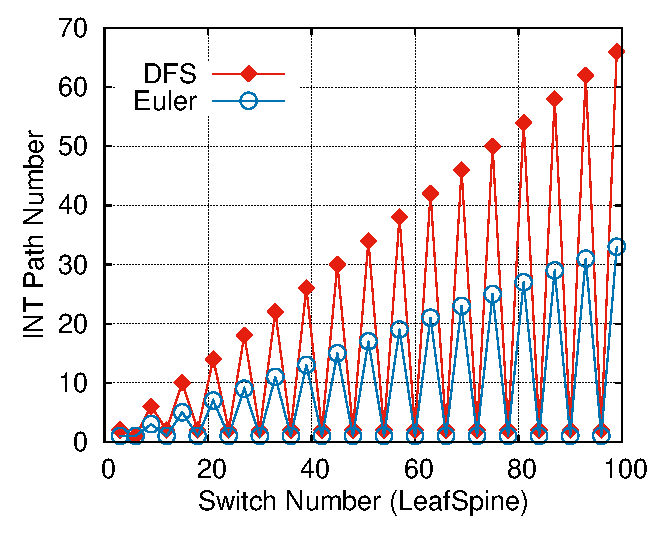
\includegraphics[width=0.23\textwidth]{figure/leaf_spine.eps}\label{fig:leaf_spine}}
\vspace{-0.15cm}
\caption{Euler outperforms DFS with classic data center network topologies.}
\label{fig:topo}
\vspace{-0.4cm}
\end{figure}

\vspace{-0.1cm}
\section{Related Work}
\vspace{-0.1cm}


% P4 协议无关转发使得有机会任意修改包头
% INT是一种P4的应用 可以采集数据平面状态,采集过程中不打扰控制平面,INT缺点
% barefoot公司的保密应用,及其问题
% 一些人也实现了 但是没有讨论
% 在2015年sigcomm有人提出pingmesh,但是主要采集endhost的实时性能数据
% 大量的应用提出基于底层数据进行ai闭环控制,但是并没有给出如何做的,我们给出了一种具体的实现方法

The proposal of INT-path builds on the giant shoulders of past researches. \cite{bosshart2014p4} invents P4, a protocol-independent packet processing architecture as well as the programming language, which enables network operators to arbitrarily modify packet headers. INT~\cite{kim2015band} is a telemetry application using P4, which can obtain device-internal states without disturbing the controller. However, INT itself is an underlying telemetry primitive for one device or a device chain without defining how to achieve network-wide telemetry, which further requires high-level orchestration. There is a very related piece of work named ``Barefoot Deep Insight'', which is also built upon INT and claims to enable \emph{end-to-end} traffic monitoring~\cite{deepinsight}. However, Barefoot Deep Insight is a proprietary solution without disclosing any technical detail. Some other works such as~\cite{van2017towards} conduct solid telemetry implementation but still do not touch the high-level orchestration. In 2015, Pingmesh~\cite{guo2015pingmesh} conducts a similar network-wide telemetry in one of Microsoft's data centers. However, Pingmesh only measures the end-host performance without diving into network devices. After all, P4 and INT are not invented at that time. As the rise of the AI age, many network AI systems claims to build closed-loop control systems depending on real-time traffic status collection~\cite{ mestres2017knowledge}. However, they talk less on the telemetry detail and our system can be a solid complement for their intelligent systems.

\section{Conclusion}

On top of the original INT primitive, we propose \emph{INT-path}, a network-wide telemetry framework/system that includes a source routing-based path monitoring mechanism and an Euler trail-based path planning policy. The mechanism allows user-specified path monitoring while the policy can \emph{optimally} generate non-overlapped INT paths that cover the entire network. Our approach can ``encode'' the network-wide traffic status into a series of ``bitmap images'', making traffic analysis as straightforward as image pattern recognition.



\small
\bibliographystyle{IEEEtran}
\bibliography{ref}
\normalsize

\end{document}
